\documentclass[parskip=half]{scrarticle}

\usepackage{amsmath}
\usepackage{graphicx}

\usepackage{listings}

\lstset{% general command to set parameter(s)
    basicstyle=\small,          % print whole listing small
    stringstyle=\ttfamily,      % typewriter type for strings
    frame=tb,
} % no special string spaces

\title{Assignment 1: Process Management}
\subtitle{CSC369H1 -- Computer Organization}

% TODO: Enter your name
\author{ZIXUAN ZENG}

\begin{document}
\maketitle

\section{Loading and running a program}

Answer the question:
``How is a program loaded and run on the Unicorn Processor?''
using 300 words or fewer.
Another way to phrase this question is ``How did you turn a program executable into a running process?''
You may include up to one figure.
Your answer should describe the sequence of steps that \textit{you} take (i.e., this should not be an answer about a generic OS), including how you interact with the data structures you have designed and their attributes.
\newline\newline\newline
Response:(figure shown in next page)\newline
 - Inside KernelCreateProcess(), Upon a call on LoadProgram() using the program path as input, it outputs the program's code, which is allocated and stored on heap, along with other info of the process(i.e. size of code, program\_entry(i.e. rip))\newline  
 - Meanwhile, a PCB is also allocated, and it stores a pointer to that code, and stores other outputs as well. Upon Process creation, PCB initializes its attributes(i.e. assigns pid, sets ProcessState  to READY, ect.), including its five registers(i.e rsp, rbp, rip, rax, rdi).\newline  
 - Then, the address of the pointer pointing at the PCB is assigned to kernel's double pointer: pcbs, which allocates a list of pointers to PCBs on the heap. \newline 
 - After that, a call on KernelRun() finds an available process' PCB from the kernel's pcbs, which is the PCB of the process that we just created, since it is initialized to READY state. It writes the text program code from PCB into CPU memory, and sets the CPU(i.e rsp, rbp, rip, rax, rdi) registers to align with PCB. \newline
 - Finally, CPUResume() runs this process in Unicorn Processor.\newline

 \newpage
\begin{figure}[ht!]
    \centering
        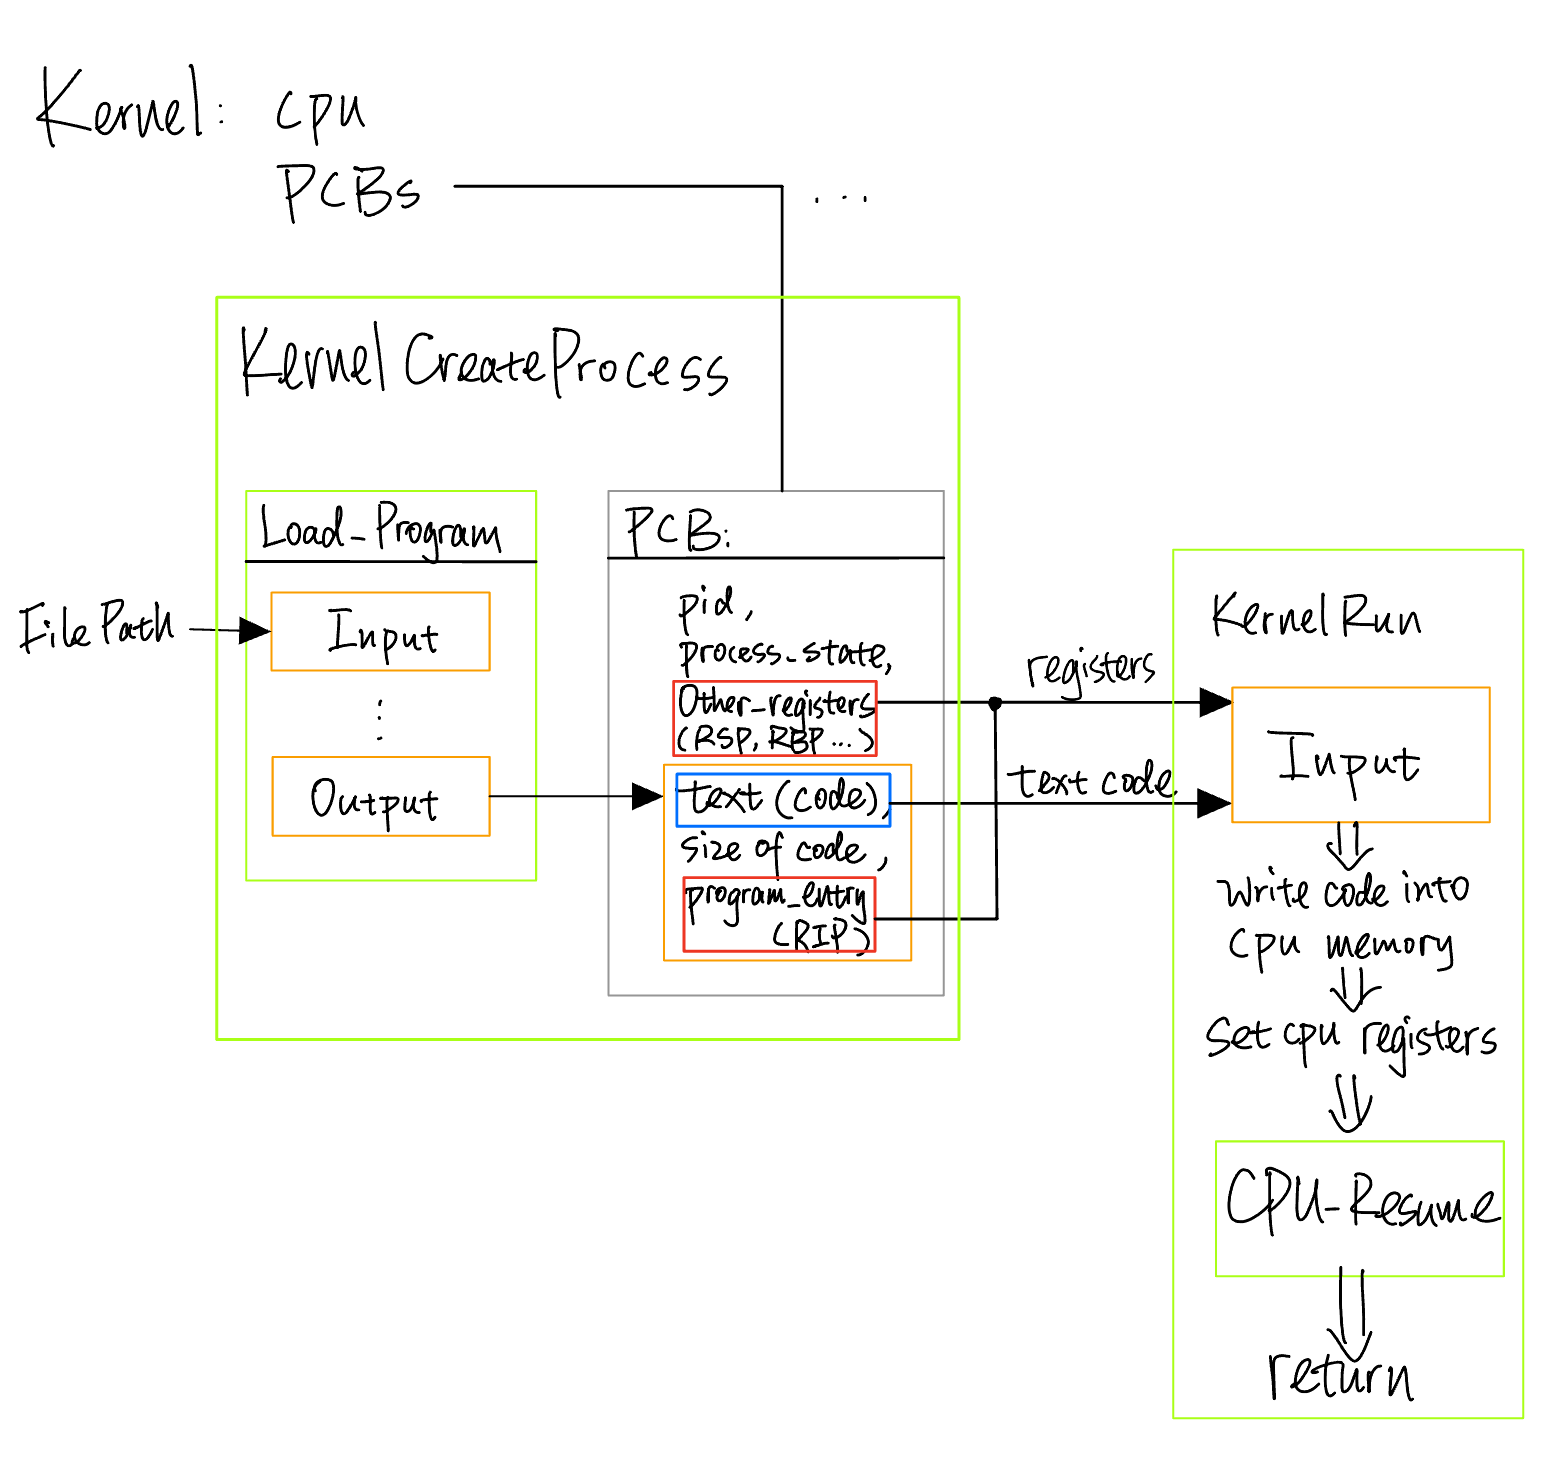
\includegraphics[width=0.7\textwidth]{figure1.png}
    \caption{exe to process pipeline}
\end{figure}

\newpage

\section{Supporting system calls}

Answer the question:
``How would you design a system call that prints a pointer to an integer?''
using 300 words or fewer.
You can assume that the pointer contains an address on the stack (since our user programs do not have a heap).
Your answer may include up to two short ``listings'' (i.e., code snippets), not included in the word count.
For example, your listings could show how the user makes the system call and how the kernel would handle the system call.
You should \textbf{not} implement this in your code.
Designing a system call to print a pointer to an integer involves two main steps: defining the system call in user space and handling the system call in kernel space.
\newline\newline\newline
Response: (code shown in next page)\newline
 - User Code:\newline Stores the pointer to integer’s value into rdi register. Sets rax register to the codex for this syscall. Then call syscall and give back control to kernel.\newline
 - Kernel Code:\newline Syscall handler decides on which syscall to execute (i.e. SystemCallPrintIntegerPointer), based on the rax register value returned and updated to PCB. Then inside the syscall function, the pointer to integer address is retrieved from the rdi register, which was also returned and updated to PCB. Then it prints the integer value using the pointer.\newline

\newpage

\begin{lstlisting}[caption=User Code System Call, label=l:userspace]
    void print_int_ptr(int *ptr) {
        register int rax __asm__ ("rax") = SYS_print_int_ptr;
        register int *rdi __asm__ ("rdi") = ptr;
        __asm__ __volatile__ (
            "syscall" 
            : "r" (rax)
            : "r" (rdi)
            : "rcx", "r11", "memory"
        )
    }
    \end{lstlisting}
    
    \begin{lstlisting}[caption=Kernel Code System Call Handler, label=l:kernelspace]
    void SystemCallPrintIntegerPointer(CSC369_Kernel* kernel) {
        assert(kernel != NULL);
        
        // Get the current process
        CSC369_PCB* pcb = kernel->curr_pcb;  // not actual implementation
        
        // retrieve rdi as pointer to int
        uc_engine* uc = CSC369_CPUExposeUnicorn(kernel->cpu);
        uc_reg_read(uc, UC_X86_REG_RDI, &pcb->rdi);
        
        // Print LOG message: integer at pointer location
        int *i = pcb->rdi;  // access integer
        CSC369_LOG_TRACE("[pid %d] CSC369_print_integer_pointer(%d)", pcb->pid, *i);
    }
    \end{lstlisting}

\newpage

\section{Process switch on exit}

Answer the question:
``How and when did you clean up a process that had finished?''
using 300 words or fewer.
You may include up to one figure.
Your answer should describe the sequence of steps that \textit{you} take (i.e., this should not be an answer about a generic OS), including how you interact with the data structures you have designed and their attributes.
\newline\newline\newline
Response:(figure shown below)\newline
 - Data Structure and Allocation:\newline Kernel, as mentioned in part 1, contains a double pointer to the PCBs: attribute pcbs points to a list of pointers on the heap, with each pointer pointing at one PCB. PCB, which is stored on the heap, contains a few attribute about the process, and a pointer to a string allocated on the heap (done by LoadProgram()). \newline
 - Clean-up Sequence:\newline When a process makes a syscall to exit, it is trapped and gives back control to the kernel. Then kernel executes this exit. First, free the space for the process’ code pointed by p\_text. Then free the PCB, which is pointed by the list of pointers pointed by pcbs. After that, the Process is cleaned up. The pointer in the list pointed by pcbs will now point to NULL. pcbs and the list it points at is remained for other processes.\newline

\begin{figure}[ht!]
    \centering
        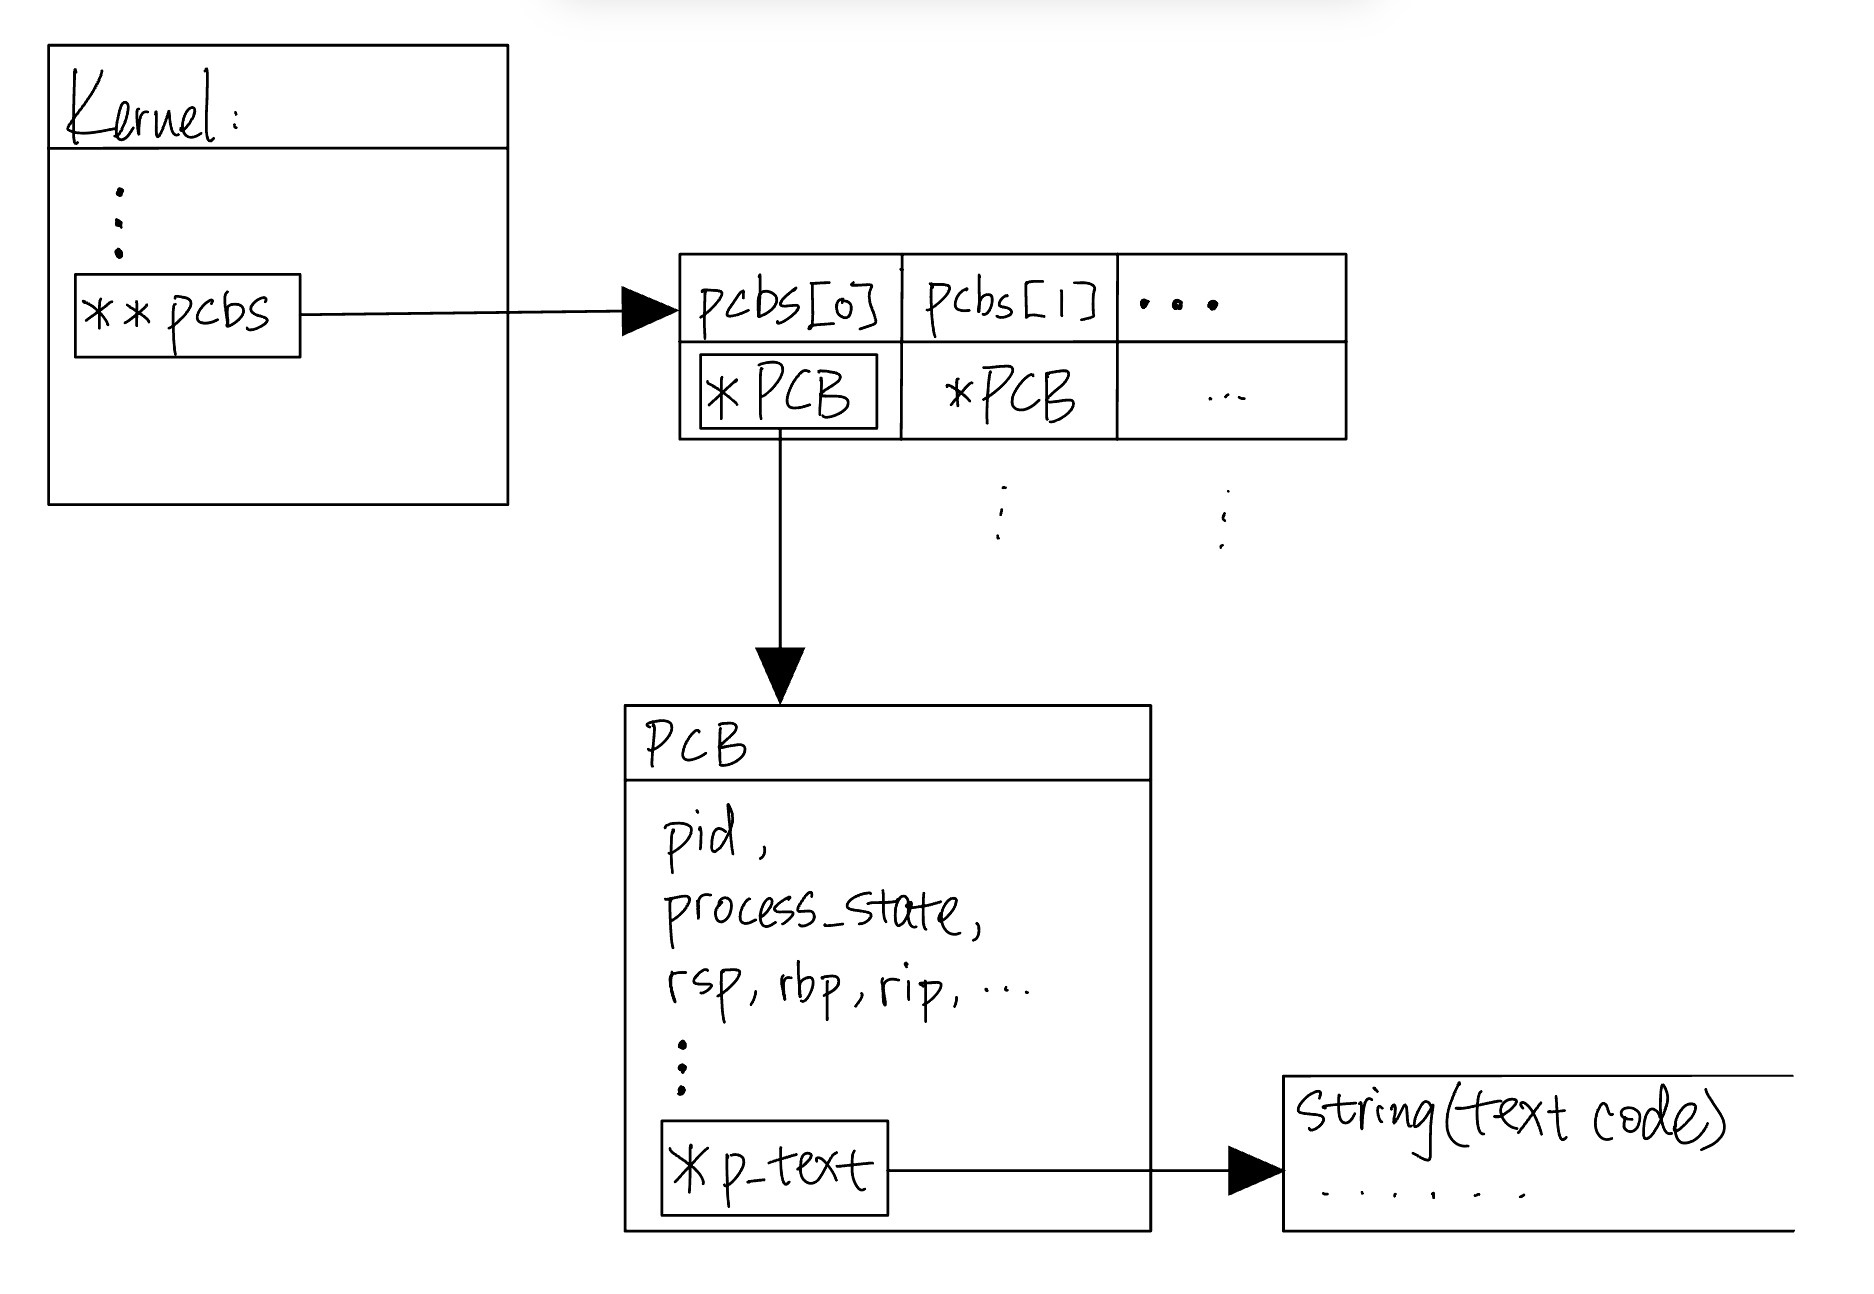
\includegraphics[width=0.8\textwidth]{figure3.png}
    \caption{PCB allocation}
\end{figure}

\newpage

\section{Cooperative process switching}

Answer the question:
``What are the different states a process in your kernel can be in, and how does a process transition between states?''
using 300 words or fewer.
You may include up to one figure.
You may find it useful to model your answer (and figure) on how it is presented in lecture or the textbook.
\newline\newline\newline

Response:(figure shown below)\newline
 - Process States:\newline BLOCKED(sudo init state), READY, RUNNING, EXIT(sudo final state).\newline
 - Process Pipeline:\newline (Note that Kernel first allocates double pointers to PCBs, initializing all state attributes to holding a blocked state. But this feature won’t be instantiated since the emulator makes sure the number of processes matches max\_procs) A sequence of processes are loaded(enqueued) into ready queue, initialized to READY state. Then processes are loaded into CPU in a Round Robin fassion. One process is dequeued from ready queue, loaded into CPU memory(cache?), and is changed to RUNNING state. On syscall, the process is changed back to READY state and then again enqueued to the ready queue (at the end). When a process makes a syscall to exit, its state is changed to EXIT (even though EXIT status does not affect program functionality). Since this process is dequeued and will never be enqueued again, it exited from the system forever.\newline

 \begin{figure}[ht!]
    \centering
        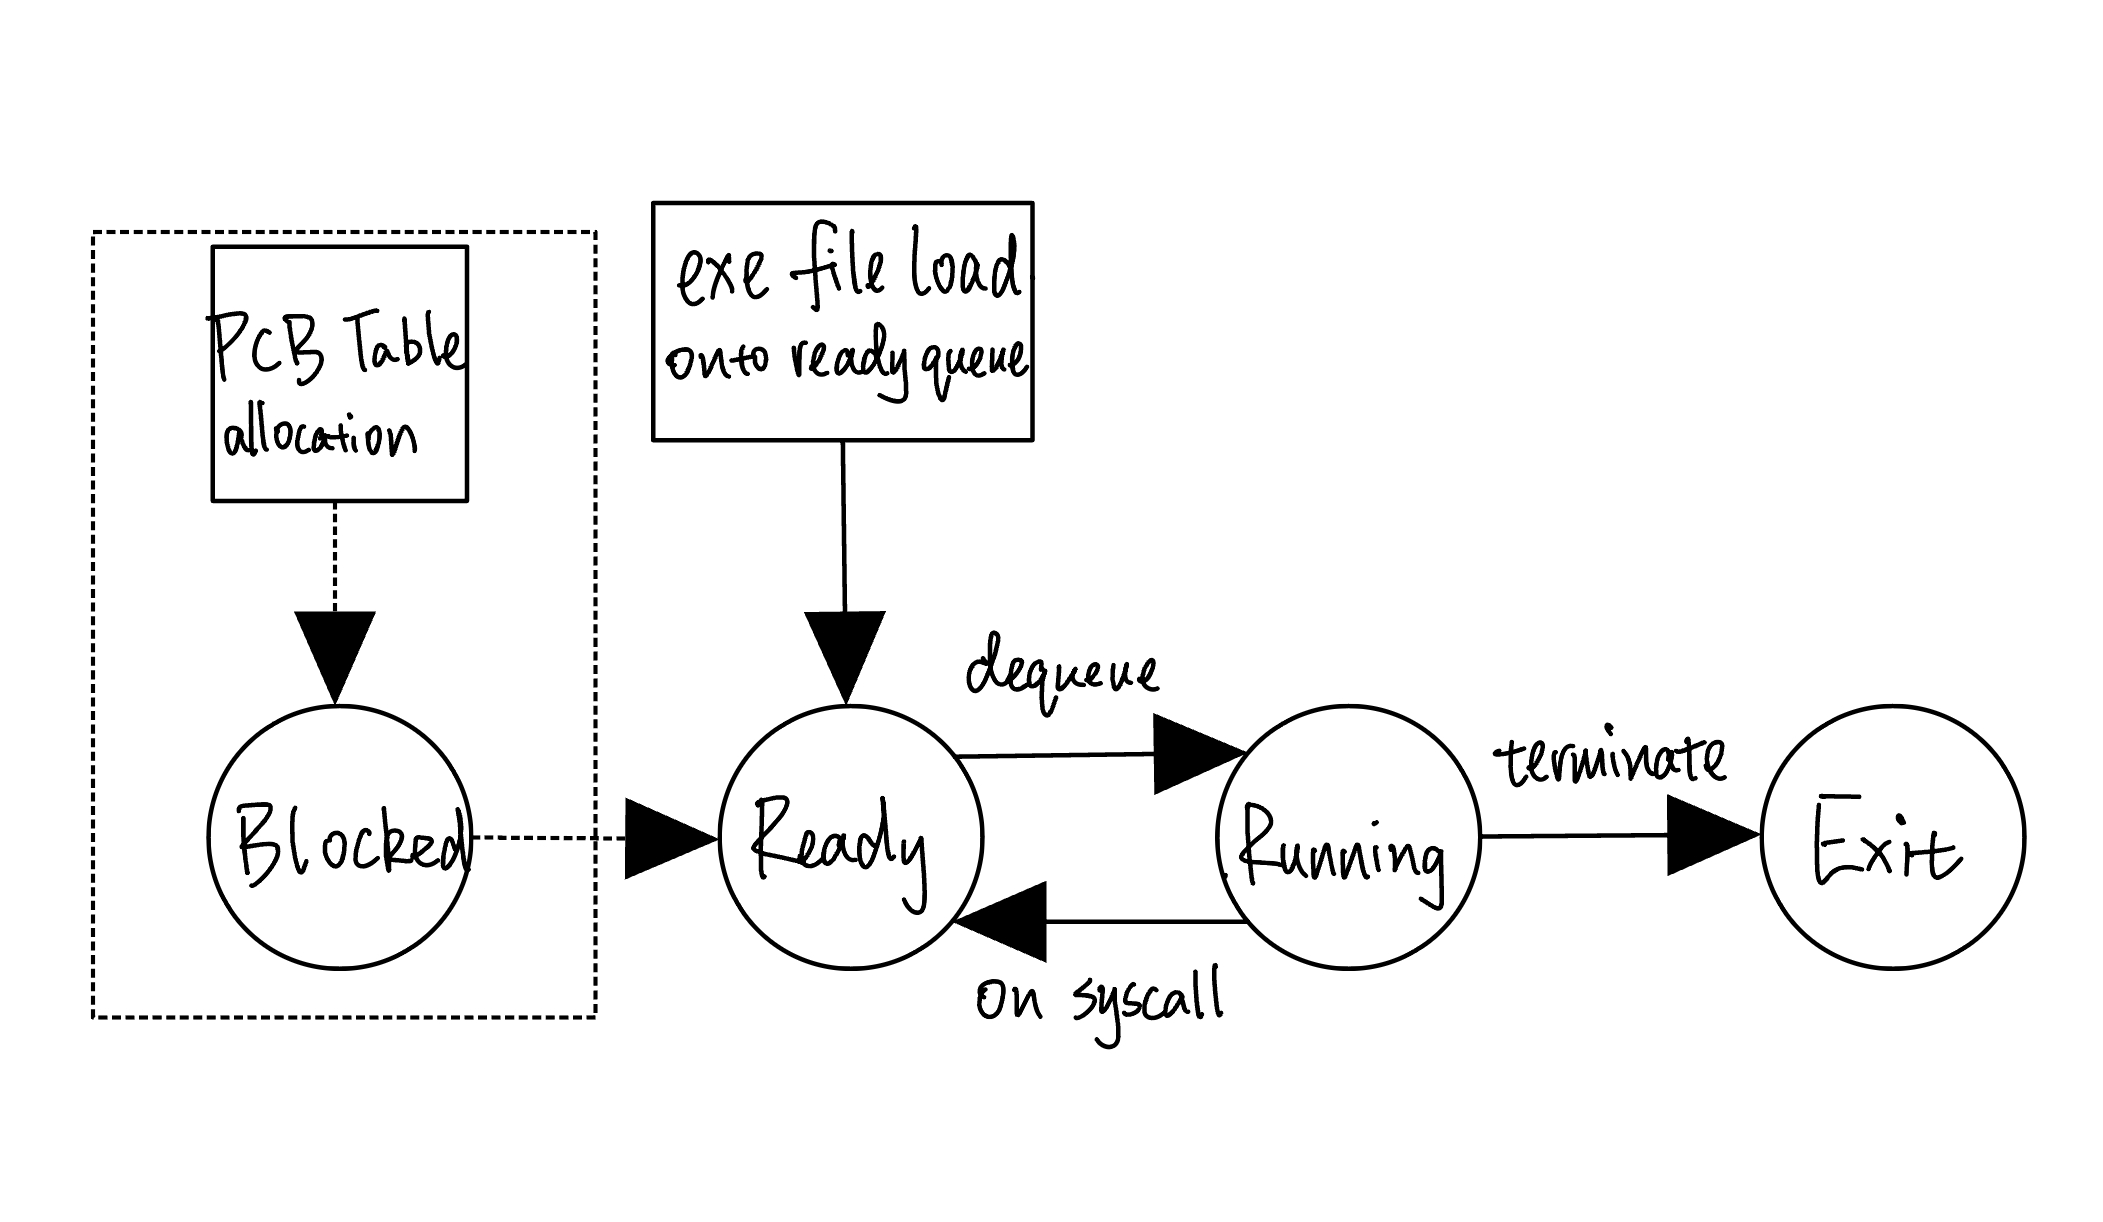
\includegraphics[width=0.8\textwidth]{figure4.png}
    \caption{TODO}
\end{figure}

\end{document}
